% !TeX root = ../../tesi.tex

\subsubsection{Clustering}
Clustering is a family of unsupervised methods aimed at grouping data samples according to \textbf{similarity} in a chosen feature space.\cite{mittal_comprehensive_2022} In image analysis, the samples typically correspond to pixels, superpixels, or local feature descriptors, while similarity may be defined in terms of color, intensity, texture, spatial position, or depth.\cite{mittal_comprehensive_2022}

Within computer vision, clustering can be exploited as a classical segmentation strategy.\cite{mittal_comprehensive_2022} The underlying idea is that pixels belonging to the same physical region often share common visual or geometric properties, and can therefore be grouped into homogeneous clusters. Once the clusters have been identified, they can be interpreted as candidate regions of interest or as a first approximation of the object masks.\cite{mittal_comprehensive_2022}

Among the simplest and most widely used approaches is \textbf{k-means clustering}, originally introduced by MacQueen,\cite{macqueen_some_1967} which partitions the input data into $k$ clusters by minimizing the within-cluster variance. When applied to images, k-means can be performed directly on RGB values, grayscale intensities, depth values, or combinations of these features.\cite{macqueen_some_1967,mittal_comprehensive_2022} This makes it particularly useful in scenarios where the target objects can be separated from the background through relatively simple low-level cues.\cite{mittal_comprehensive_2022}

In the present work, clustering is relevant because dough segmentation can benefit from the grouping of pixels or 3D points with similar visual or geometric properties. In the considered setup, color and depth cues can facilitate the separation between the dough and the surrounding scene. In this sense, clustering can be considered a useful classical tool for preprocessing, exploratory segmentation, or the extraction of candidate regions in controlled industrial environments.\cite{mittal_comprehensive_2022}
\begin{figure}[h]
    \centering
    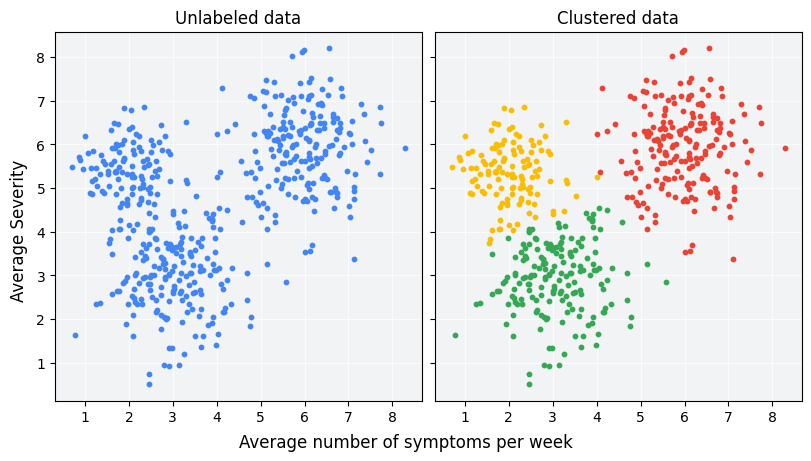
\includegraphics[scale=0.4]{images/clustering.png}
    \caption{Visualization of k-means clustering applied to an image, where pixels are grouped into clusters based on their similarity and distance in the feature-space. Each cluster is represented by a different color, illustrating how the algorithm partitions the image into distinct regions.}
    \label{fig:clustering}
\end{figure}


\subsubsection{Background subtraction}
Background subtraction is another classical strategy for foreground extraction. The main idea is to maintain a model of the background and compare the current observation against it, so as to identify the regions that differ significantly from the static part of the scene.\cite{opencv_background_subtraction_2026}

In vision-based applications, this approach is commonly used with static cameras to generate a foreground mask, that is, a binary image containing the pixels associated with the moving or changing objects in the scene.\cite{opencv_background_subtraction_2026} More generally, the same principle can be extended to cases in which the background is known or can be estimated in advance, and the goal is to isolate the objects of interest by removing the supporting surface or the stationary scene structure.
\begin{figure}[h]
    \centering
    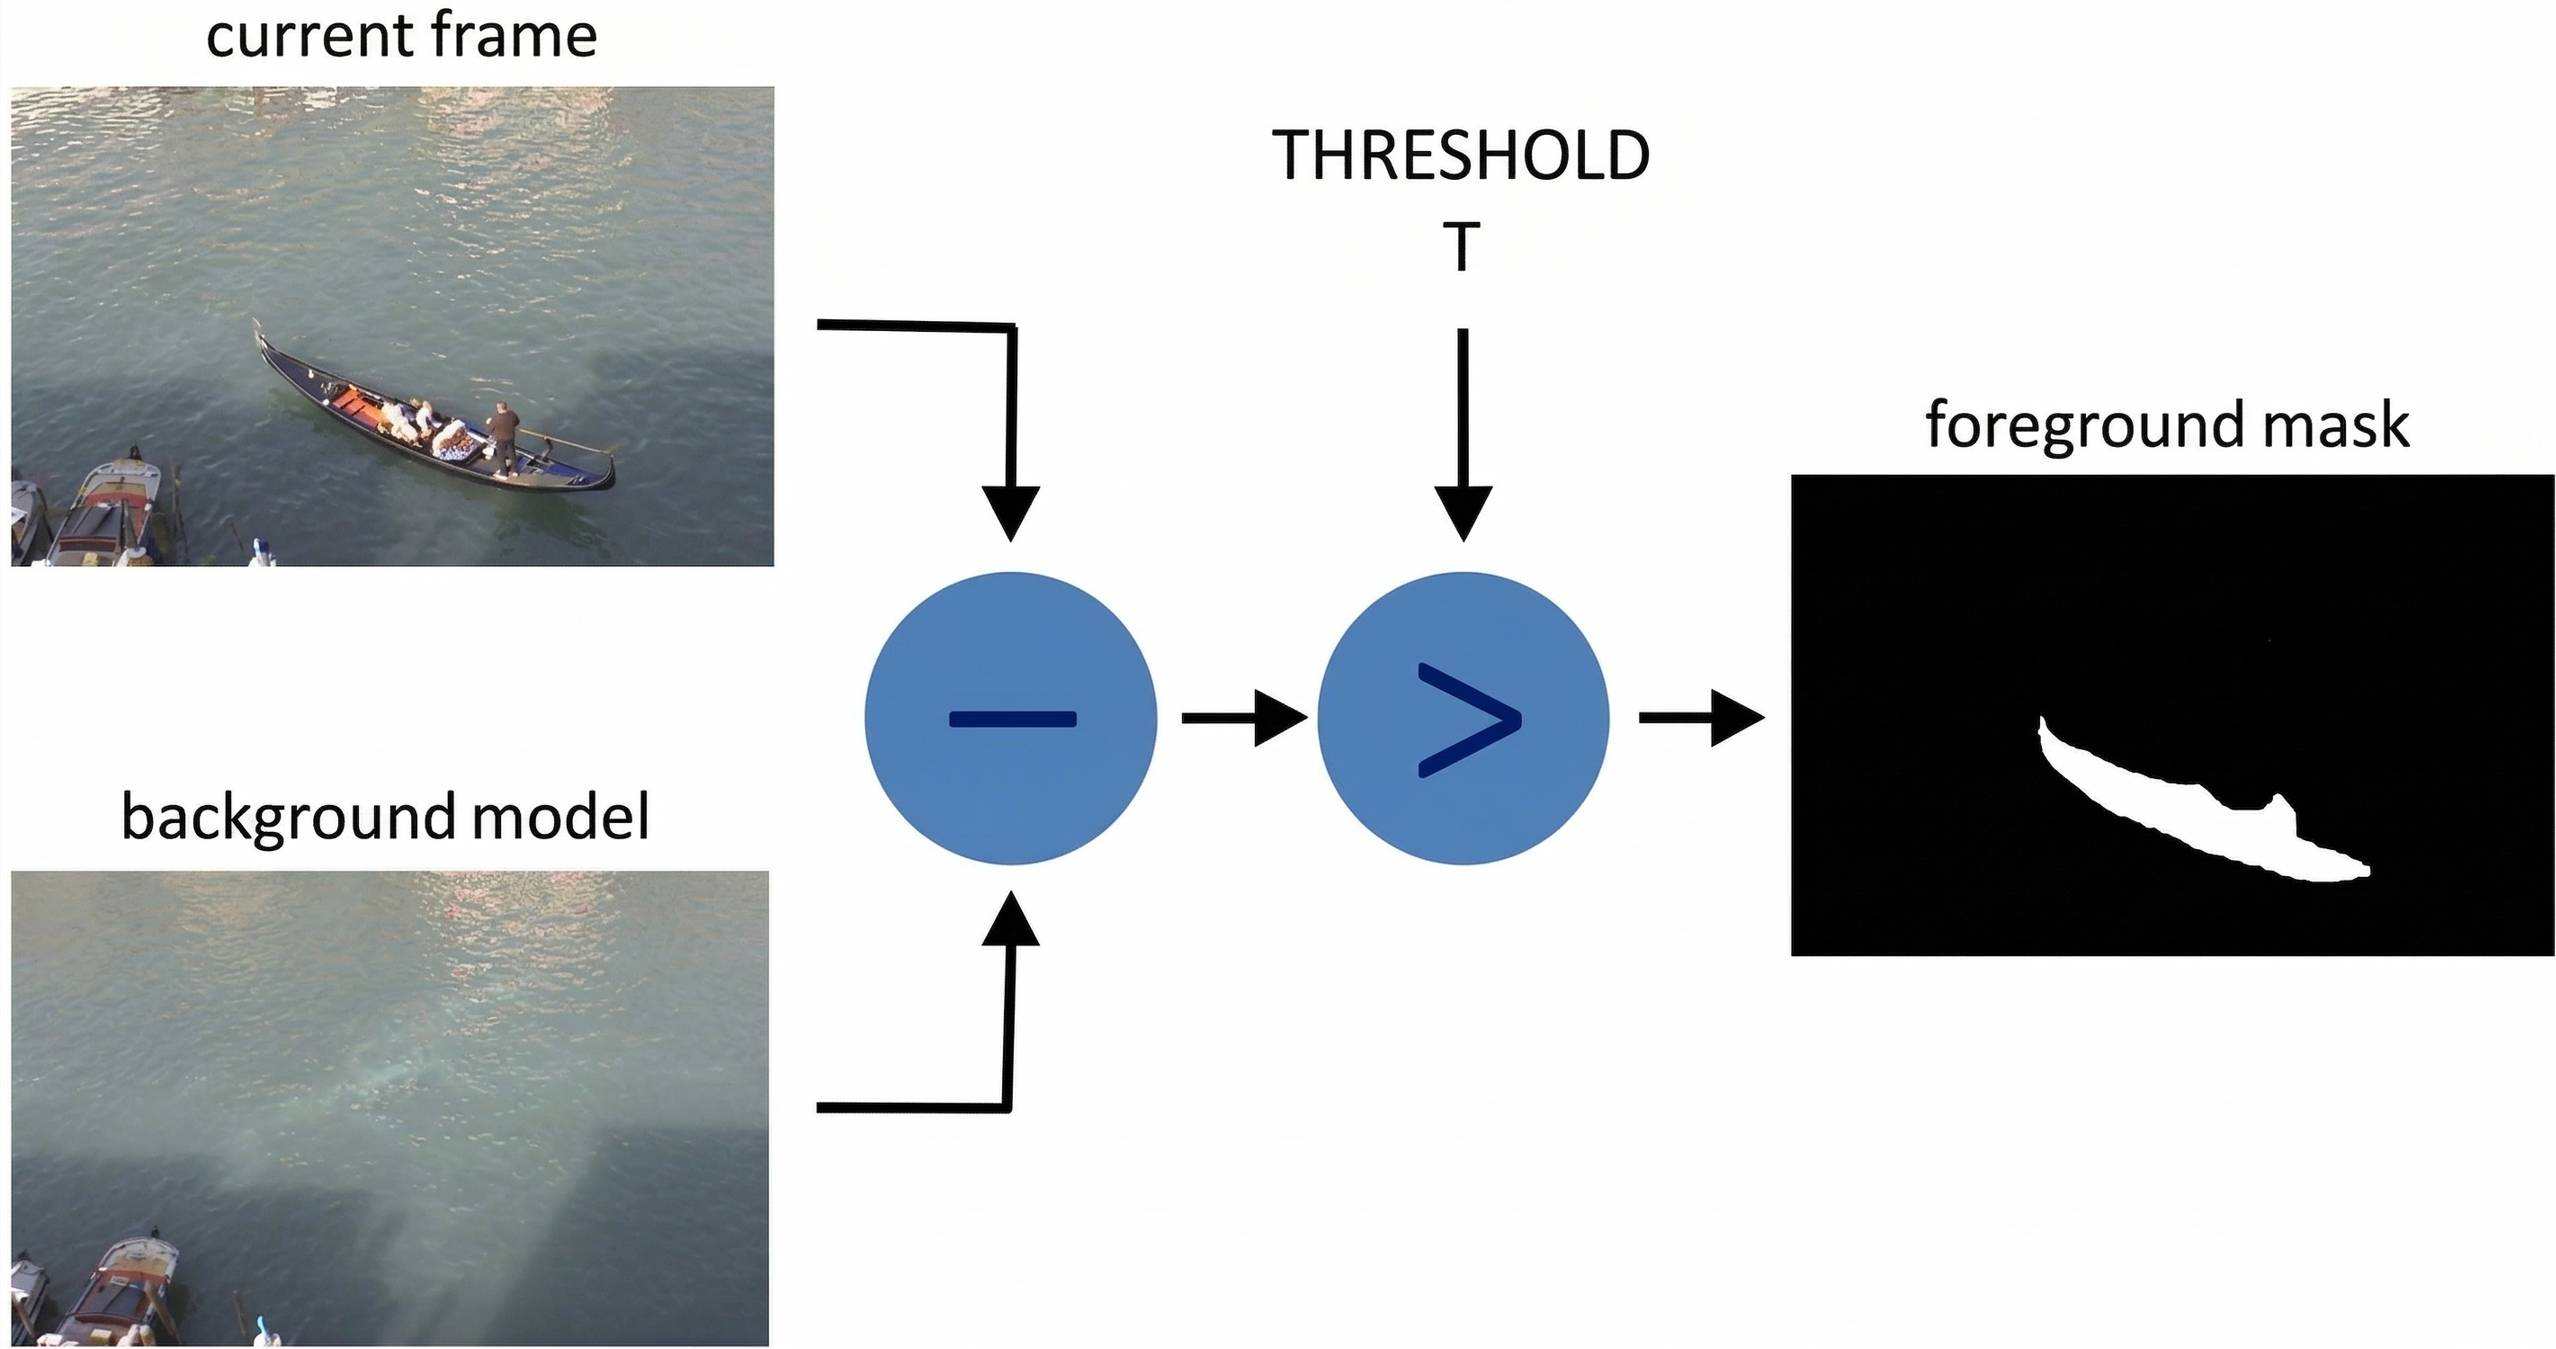
\includegraphics[width=0.6\textwidth]{images/Background_subtraction.png}
    \caption{Background subtraction example scheme.}
    \label{fig:background-subtraction}
\end{figure}

In the present work, this idea is relevant in two complementary ways. First, background subtraction is used in a non segmentation context in the RGB stream as part of the motion-detection module for dataset acquisition. Second, a conceptually similar foreground-background separation is exploited on depth information to isolate the dough from the supporting table before the subsequent geometric analysis.
Since the background (table) is static and can be reliably estimated in depth, this approach provides a computationally efficient way to segment the dough units without relying on complex learning-based models, which may be unnecessary in this controlled setting.
